
\section{Problems of classical I2A}
\begin{frame}{Problems of classical I2A}
    \begin{PraesentationAufzaehlung}
        \item Not scalable to large observations -- rollouts are slow
        \item Not scalable to large action spaces -- one rollout per action
        \item Environment model has problems predicting far into the future
    \end{PraesentationAufzaehlung}
\end{frame}

\begin{frame}
	\frametitle{Classical I2A rollout}
	\vspace{-10mm}
	\begin{multicols}{2}
	\begin{figure}[h]
		\centering
		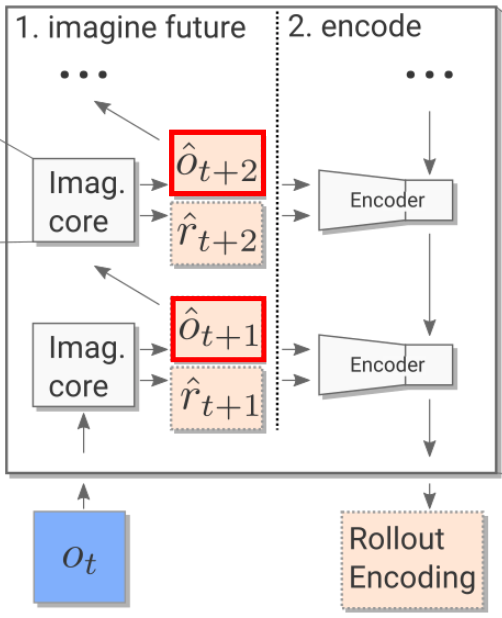
\includegraphics[height=0.65\textheight]{./latent_i2a_images/SingleImaginationRollout_marked.png}
	\end{figure}
	\columnbreak
	\centering
	$\mathnormal{o_t \rightarrow s_t \rightarrow \hat{o}_{t+1}}$\\
	$\mathnormal{\hat{o}_{t+1} \rightarrow s_{t+1} \rightarrow \hat{o}_{t+2}}$\\
	...
	\end{multicols}
\end{frame}

\begin{frame}{Solution to large observations}
	\begin{PraesentationAufzaehlung}
	    \item Compress observation into a latent representation
	    \item Compute rollout based on compressed state not on images\\
	    $\mathnormal{o_t \rightarrow s_t}$\\
	    $\mathnormal{s_t \rightarrow s_{t+1}}$\\
	\end{PraesentationAufzaehlung}
\end{frame}


%reference to 2nd paper
\begin{frame}
	\frametitle{Relevant Papers}
\begin{PraesentationAufzaehlung}
    \item Imagination-Augmented Agents for Deep Reinforcement Learning, Weber et al.(2017)
	\vspace{20mm}
    \item Learning and Querying Fast Generative Models for Reinforcement Learning, Buesing et al.(2018)
\end{PraesentationAufzaehlung}

\end{frame}
\clearpage


%reminder of classical rollout structure
\begin{frame}
	\frametitle{Classical I2A rollout}
	\begin{figure}[h]
		\centering
		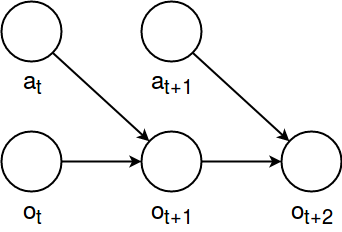
\includegraphics[height=0.5\textheight]{./latent_i2a_images/Classic_I2A_Rollout.png}
	\end{figure}
\end{frame}

%dSSM-DET
\begin{frame}
	\frametitle{dSSM-DET}
	\vspace{-10mm}
	deterministic State Space Model - Deterministic
	\begin{multicols}{2}
		\begin{figure}[h]
			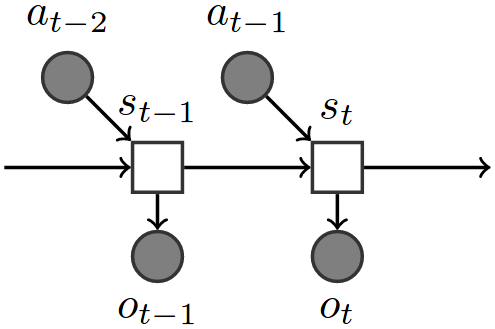
\includegraphics[width=0.4\textwidth]{./latent_i2a_images/dSSM_DET_architecture.png}	
		\end{figure}
		\columnbreak
		$s_t$: compact latent representation of observation at time t\\
		$a_t$: action at time t\\
		$o_t$: predicted output
	\end{multicols}
%	\vfill
%	
%	\footnotesize
%   Images for this and the next 2 slides taken from Learning and Querying Fast Generative Models for Reinforcement Learning, Buesing et al.(2018)
%\normalsize 
\end{frame}

%dSSM-VAE
\begin{frame}
	\frametitle{dSSM-VAE}
	\vspace{-10mm}
	deterministic State Space Model - Variational Autoencoder
	\begin{multicols}{2}
		\begin{figure}[h]
			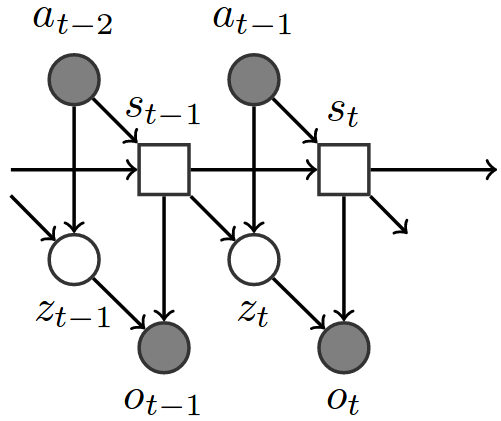
\includegraphics[width=0.4\textwidth]{./latent_i2a_images/dSSM_VAE_architecture.png}	
		\end{figure}
		\columnbreak
		$z_t$: latent variable\\
		 sampled from gaussian distribution given by learnable mean and standard deviation (based on $s_{t-1}$ and $a_{t-1}$)
		\textbf{Decoder} depends on $z_t$
	\end{multicols}
\end{frame}


%closer examination of sSSM - dSSM types can be seen as subtypes of sSSM
\begin{frame}
	\frametitle{sSSM}
	\vspace{-10mm}
	stochastic State Space Model\\
	dSSM variants can be seen as simplifications of sSSM \\
	\begin{multicols}{2}
		\begin{figure}[h]
			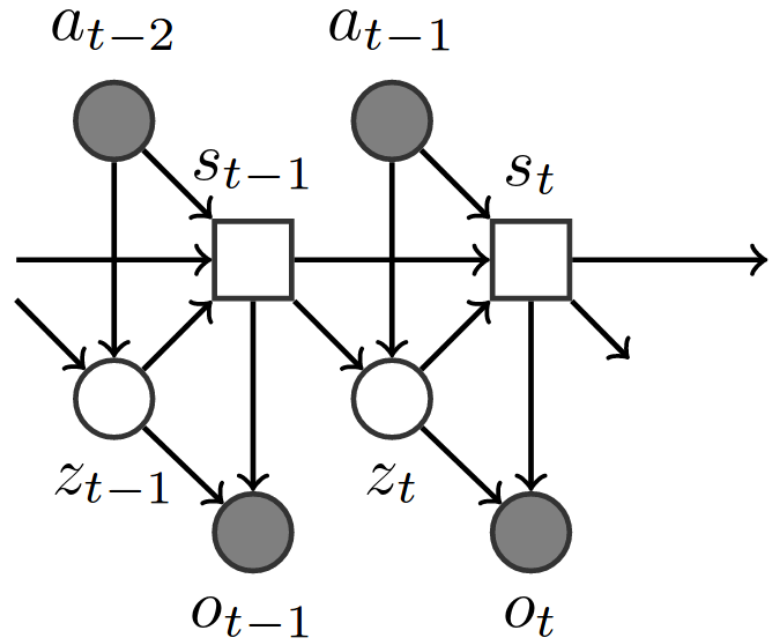
\includegraphics[width=0.4\textwidth]{./latent_i2a_images/sSSM2.png}	
		\end{figure}
		\columnbreak
		\begin{PraesentationAufzaehlung}
			\item Now the \textbf{transition and the decoder} depend on the sampled latent variable
			\item Explicitly models uncertainty of state $s_{t+1}$
		\end{PraesentationAufzaehlung}
	\end{multicols}
\end{frame}


\begin{frame}
	\frametitle{State Space Models}
	\begin{PraesentationAufzaehlung}
		\item dSSM-DET  (deterministic State Space Model, deterministic decoder) 
		\vspace{10mm}
		\item dSSM-VAE (deterministic State Space Model, stochastic decoder)
		\vspace{10mm}
		\item sSSM (stochastic State Space Model, stochastic decoder)
	\end{PraesentationAufzaehlung}
\end{frame}

\begin{frame}
	\frametitle{Environment Model Encoder}
	\begin{figure}[h]
		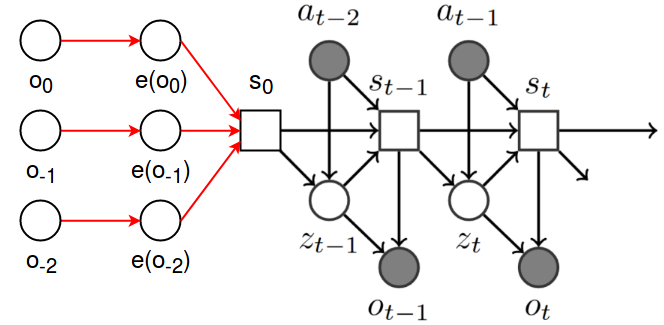
\includegraphics[width=0.8\textheight]{./latent_i2a_images/Encoder.png}	
	\end{figure}
	\begin{PraesentationAufzaehlung}
		\item encoding via space-to-depth operation and conv-stacks
		\item $s_0$ is based on the 3 previous encodings
	\end{PraesentationAufzaehlung}
\end{frame}

\begin{frame}
	\frametitle{Environment Model Decoder}
	\begin{multicols}{2}
		\begin{figure}[h]
			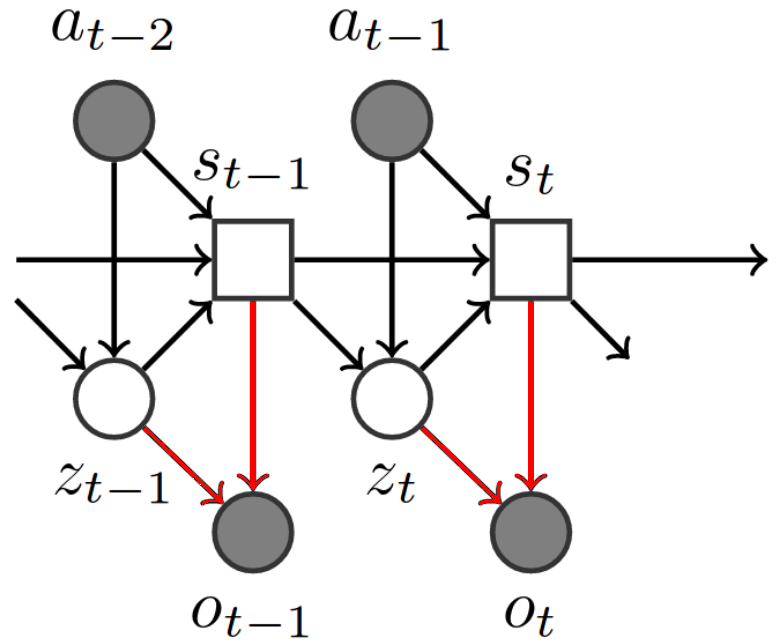
\includegraphics[width=0.4\textwidth]{./latent_i2a_images/sSSM2_decoder_marked.png}	
		\end{figure}
		\columnbreak
		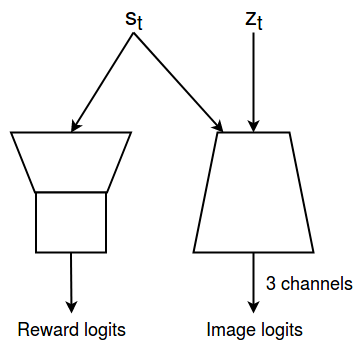
\includegraphics[width=0.4\textwidth]{./latent_i2a_images/LatentSpaceDecoder.png}
	\end{multicols}
\end{frame}

\begin{frame}
	\frametitle{Environment Model State Transition}
	\begin{multicols}{2}
		\begin{figure}[h]
			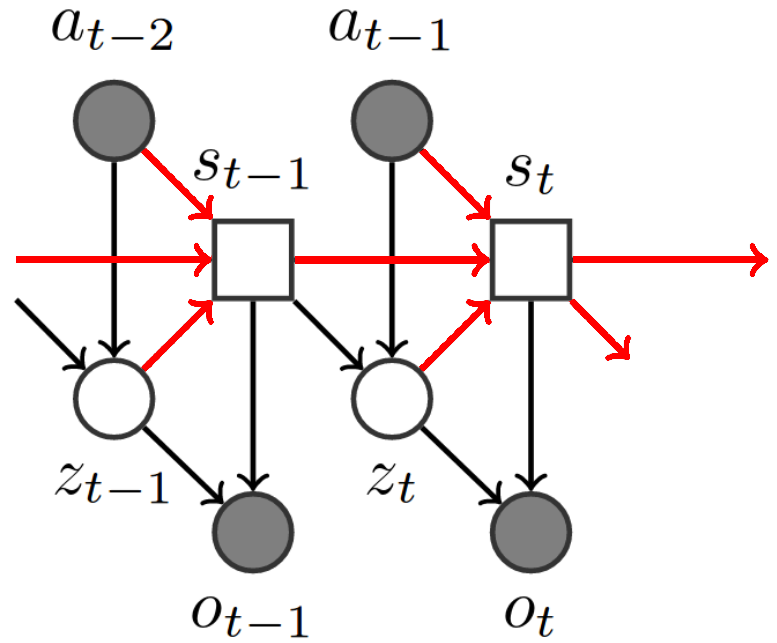
\includegraphics[width=0.4\textwidth]{./latent_i2a_images/sSSM2_state_transition_marked.png}	
		\end{figure}
		\columnbreak
		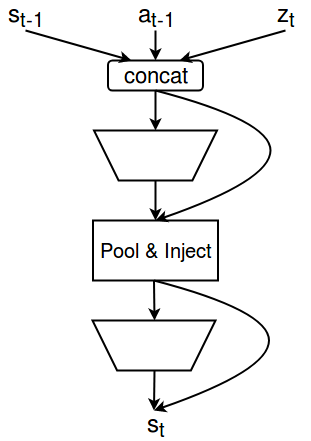
\includegraphics[width=0.4\textwidth]{./latent_i2a_images/LatentSpaceTransition.png}
	\end{multicols}
\end{frame}


\begin{frame}{Training the dSSM-DET Model}
    Maximum Likelihood Estimation:
    \begin{equation}
    \mathnormal{
            L(\theta) = \log p_{\theta}(o_{1:T}|a_{0:T-1}, \hat{o}_0)}
    \end{equation}
        $\hat{o}_0$: initial context\\
        the encodings of the last 3 observations are used to generate $s_0$ in a learnable way
    
\end{frame}

\begin{frame}{Training the sSSM Model}
		\begin{PraesentationAufzaehlung}
			\item We cannot directly evaluate $\mathnormal{L(\theta)}$ when using latent variables as it depends on the posterior $\mathnormal{p(z_t|s_{t-1},a_{t-1})}$
			\item Approximate true posterior $\mathnormal{p(z_t|s_{t-1},a_{t-1})}$ with approximated posterior $\mathnormal{q(z_t|s_{t-1},a_{t-1},o_{t:T})}$
			\item Use Kullback-Leibler divergence
			\begin{equation}
			\mathnormal{
			\begin{aligned}
			KL(q(z_t|s_{t-1},a_{t-1},o_{t:T})|p(z_t|s_{t-1},a_{t-1})) \\= \int q(z_t|s_{t-1},a_{t-1}) \log \frac{q(z_t|s_{t-1},a_{t-1},o_{t:T})}{p(z_t|s_{t-1},a_{t-1})}dz
			\end{aligned}	
			}		
			\end{equation}
			\item Reformulate as Evidence Lower Bound (ELBO)
		\end{PraesentationAufzaehlung}
\end{frame}

\begin{frame}
	\frametitle{Training the sSSM Model}
		\vspace{-10mm}
        Evidence Lower Bound:
        \begin{equation}
		\mathnormal{
        \begin{aligned}
            ELBO_q(\theta) = \sum_{t=1}^T \EX_q[\log p(o_t|s_t) + \log p(z_t|s_{t-1}, a_{t-1})\\ - \log q(z_t|s{t-1}, a_{t-1}, o_t)]
        \end{aligned}
		}
        \end{equation}
        
        ELBO = reconstruction loss + KL-Div between true and approximated posterior\\
        \vspace{10mm}
        \href{https://jaan.io/what-is-variational-autoencoder-vae-tutorial/}{https://jaan.io/what-is-variational-autoencoder-vae-tutorial/}
\end{frame}

\begin{frame}
	\frametitle{Reconstruction loss}
	$\mathnormal{p(o_t|s_t)}$: Bernoulli Distribution \\
        $\rightarrow$ Compute reconstruction loss with binary cross entropy\\
        \vspace{10mm}
	How can the image output be Bernoulli distributed?
        \begin{PraesentationAufzaehlung}
        	\item Interpret channels of decoder output scaled between 0 and 1 as probabilities of a Bernoulli distribution
        	
        \end{PraesentationAufzaehlung}
\end{frame}

\begin{frame}
	\frametitle{Reward prediction}
	\begin{PraesentationAufzaehlung}
		\item Binary representation of the reward
		\begin{equation}
			\mathnormal{
			\sum_{n=0}^{N-1}b_{t,n}2^n = \lfloor r_t \rfloor
			}
		\end{equation}
		\item Bits are modeled as independent Bernoulli variables
		\item 2 additional bits: sign and zero indicator
	\end{PraesentationAufzaehlung}
\end{frame}


\begin{frame}
	\frametitle{Comparison of Environment Model architectures}
	\begin{PraesentationAufzaehlung}
		\item Stochastic architectures perform better at predicting the future\\
		\item I2A seems to have difficulties learning from the output of sSSM
		\item dSSM-DET performs best when combining it with I2A
	\end{PraesentationAufzaehlung}
\end{frame}




\begin{frame}{dSSM-DET rollout prediction}
    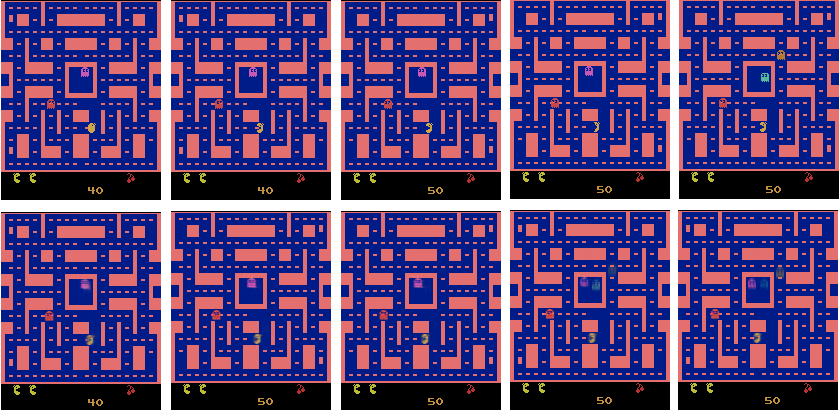
\includegraphics[width=\textwidth]{./latent_i2a_images/dSSM_rollout_prediction.png}
\end{frame}

%TODO video
\begin{frame}
	\frametitle{sSSM rollout prediction demo}
\end{frame}


\begin{frame}
	\frametitle{Why is MsPacman a hard prediction problem?}
	\begin{PraesentationAufzaehlung}
		\item Observation size: 160x200x3
		\item Sprites of pacman and ghosts are not static
		\item Blinking objects, essential objects are not seen in all frames
		\item Ghosts follow certain rules -- the environment model has to learn them to predict ghost behaviour
		\item Some reward-types are very sparse
	\end{PraesentationAufzaehlung}
\end{frame}

    
\begin{frame}{Environment Model training loss}
	\vspace{-10mm}
   	\begin{figure}
       \centering
        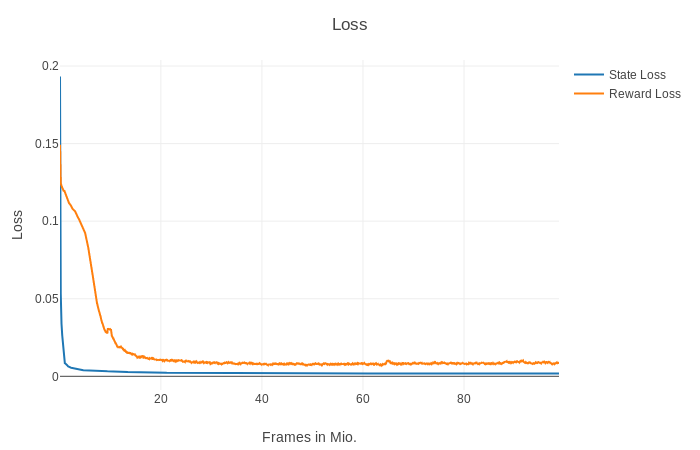
\includegraphics[width=0.9\textwidth]{./latent_i2a_images/EnvironmentModel_dSSM-DET_training.png}
    \end{figure}
\end{frame}





\begin{frame}
	\frametitle{Original I2A architecture}
	\begin{figure}
        \centering
        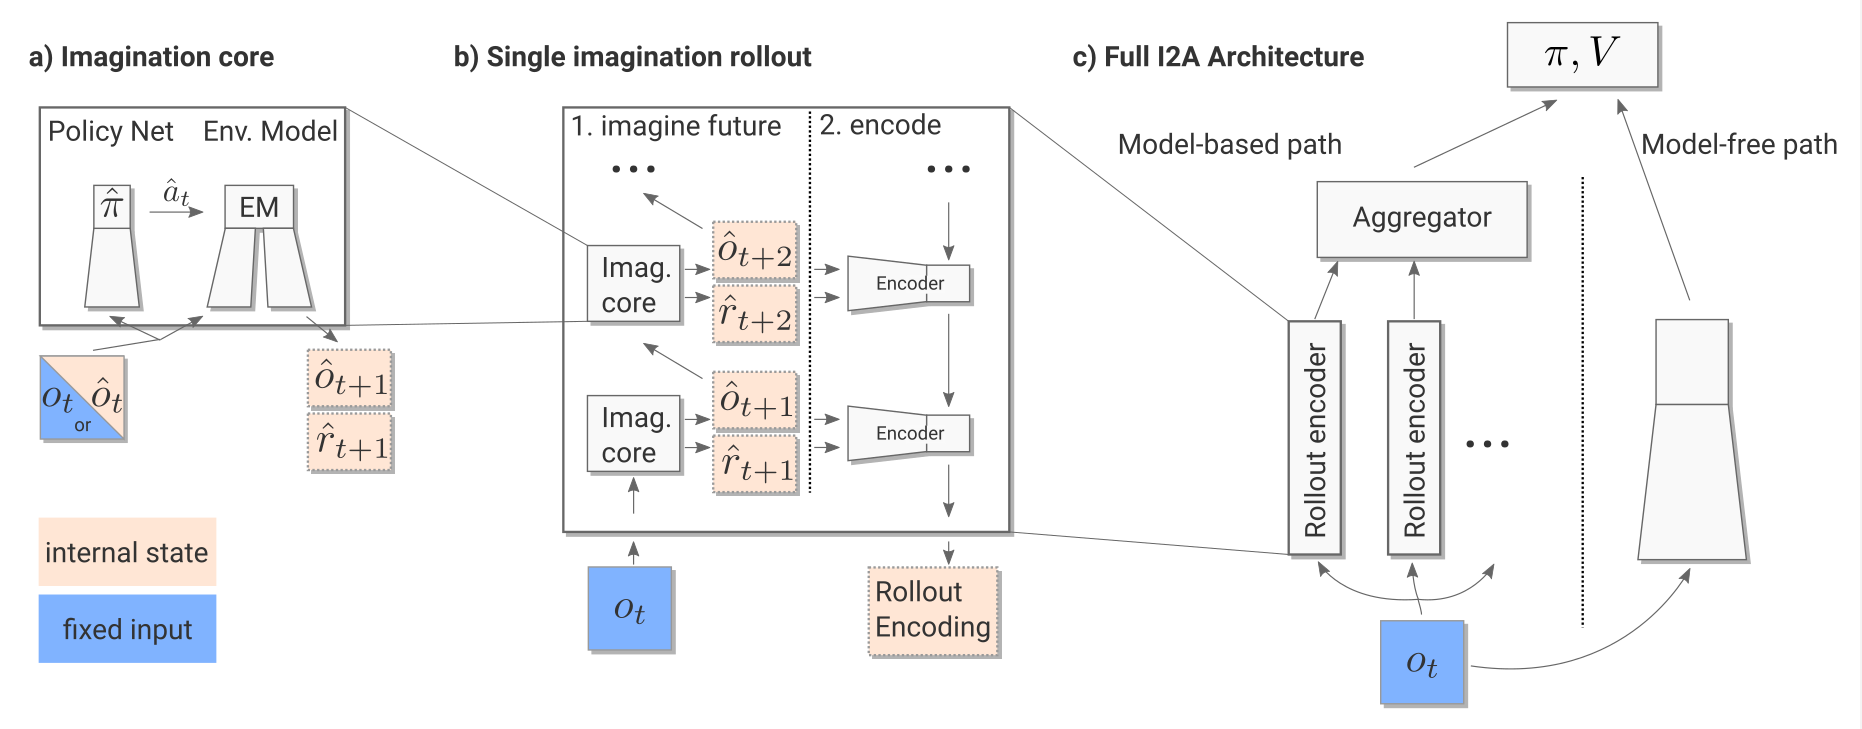
\includegraphics[width=\textwidth]{./latent_i2a_images/i2a_architecture.png}
    \end{figure}
\end{frame}

\begin{frame}
	\frametitle{Modified I2A architecture}
	\begin{figure}
        \centering
        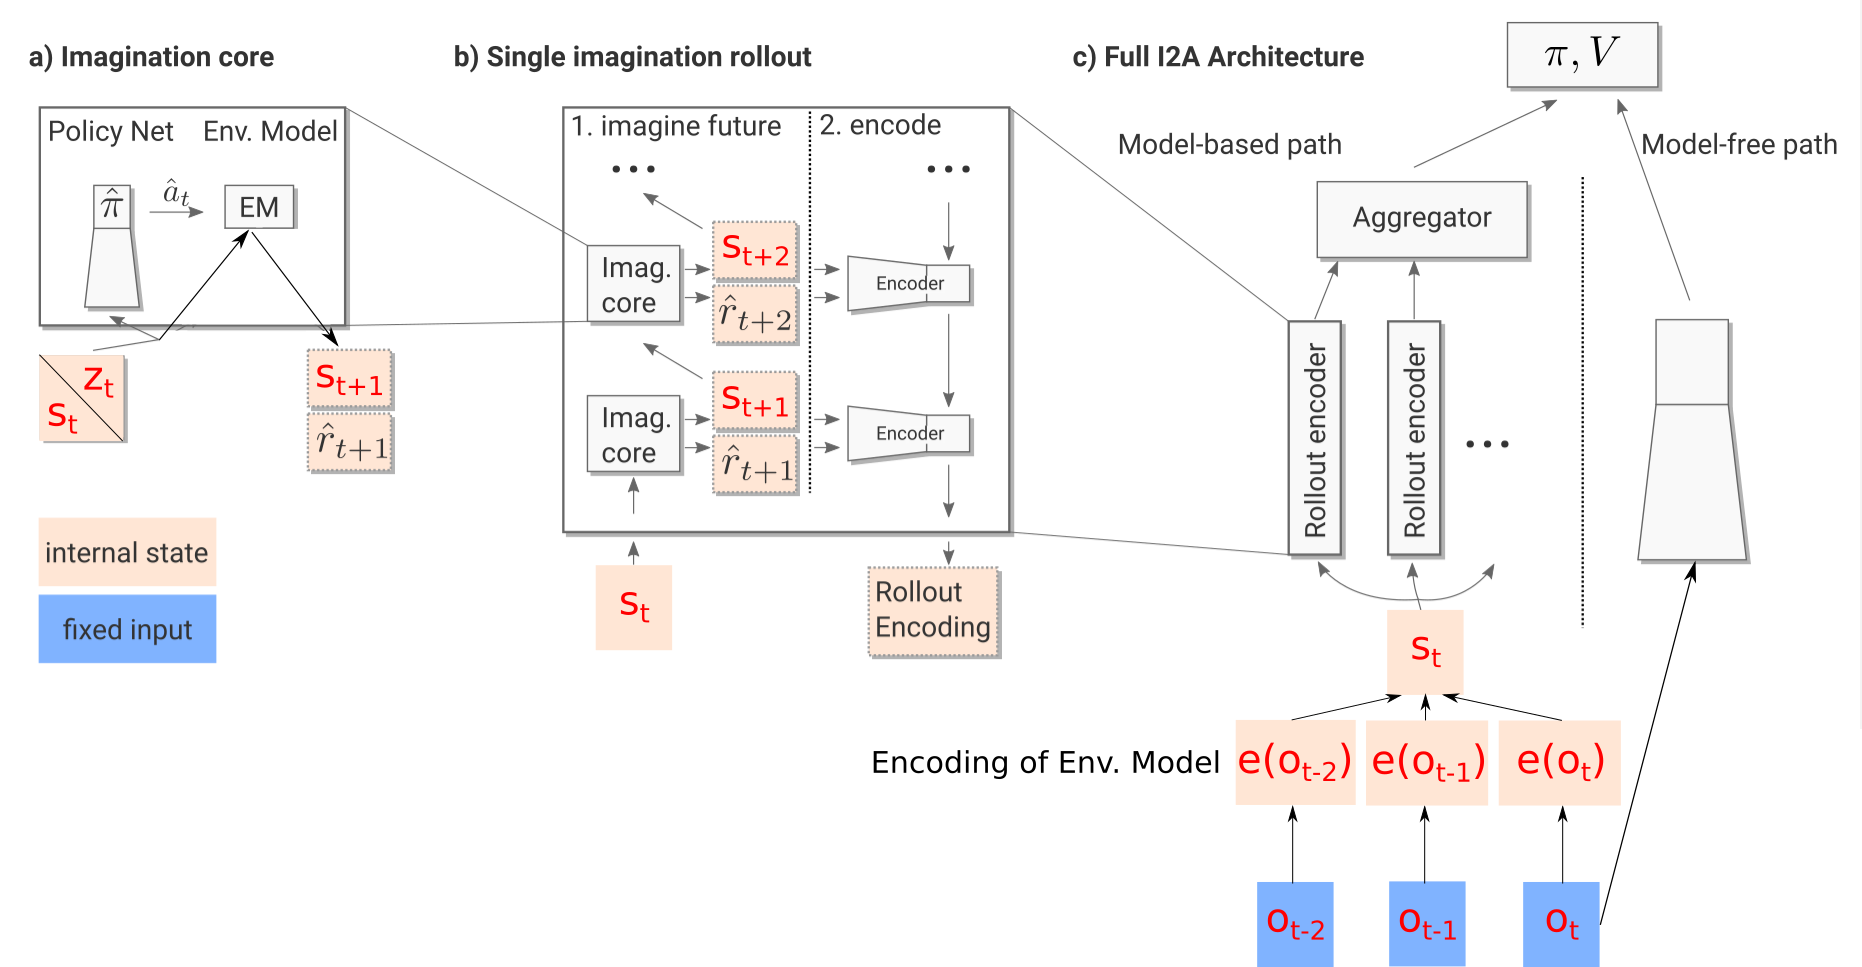
\includegraphics[width=\textwidth]{./latent_i2a_images/latent_i2a_architecture_finished3.png}
    \end{figure}
\end{frame}


%results on MsPacman
\begin{frame}
	\frametitle{Why is MsPacman a hard reinforcement learning problem?}
	\begin{PraesentationAufzaehlung}
		\item The Agent needs to plan into the future $\rightarrow$ I2A
		\item The input is a raw image -- the agent initially knows nothing about objects $\rightarrow$ Conv-Layers, Latent Space I2A
		\item Large observations $\rightarrow$ Latent Space I2A
		\item Dense rewards (eat), that do not help much in learning the way to get large (sparse) rewards fast (power pills, kill ghosts)
	\end{PraesentationAufzaehlung}
\end{frame}

\begin{frame}
	\frametitle{MsPacman}
	\begin{PraesentationAufzaehlung}
		\item Environment MsPacmanNoFrameskip-v0 from OpenAI Gym
		\item Original input size: (210, 160, 3) cropped to (200, 160, 3)
	
		\item Reward:\\
		\vspace{5mm}
		\hspace{-4mm}
		\begin{tabular}{ p{7cm}  r }
	  	Eating food & 10 \\
		Eating power pill & 50\\
		Eating ghost & 200,400,800,1600\\
		Killed by ghost & -100\\
		Eating Fruits & 100-5000\\
		\end{tabular}
		\vspace{5mm}
		\item Fruit rewards are extremely sparse and higher value fruits only appear in later levels.
	\end{PraesentationAufzaehlung}
\end{frame}

\begin{frame}
	\frametitle{Specifics of I2A run of MsPacman}
	\begin{PraesentationAufzaehlung}
		\item Environment Model: dSSM\_DET
		\item Optimizer: RMSProp, learning rate=7e-4
		\item Framestack: 4
		\item Frameskip: 4
		\item Distill coefficient: 10
		\item Entropy coefficient: 0.02
		\item Rollout length: 2, 5
	\end{PraesentationAufzaehlung}
\end{frame}

\begin{frame}{dSSM-DET MsPacman rollout length 2}
	\vspace{-10mm}
    \begin{figure}
        \centering
        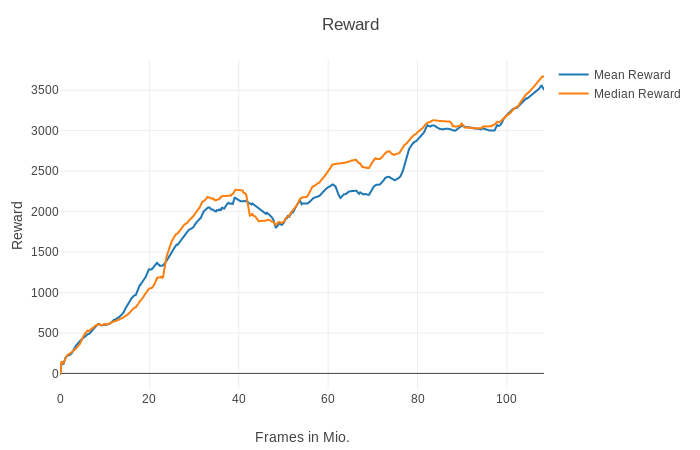
\includegraphics[width=0.9\textwidth]{./latent_i2a_images/dSSM_DET_MsPacman_100mio.png}
    \end{figure}
\end{frame}

\begin{frame}{dSSM-DET MsPacman rollout length 5}
	\vspace{-10mm}
    \begin{figure}
        \centering
        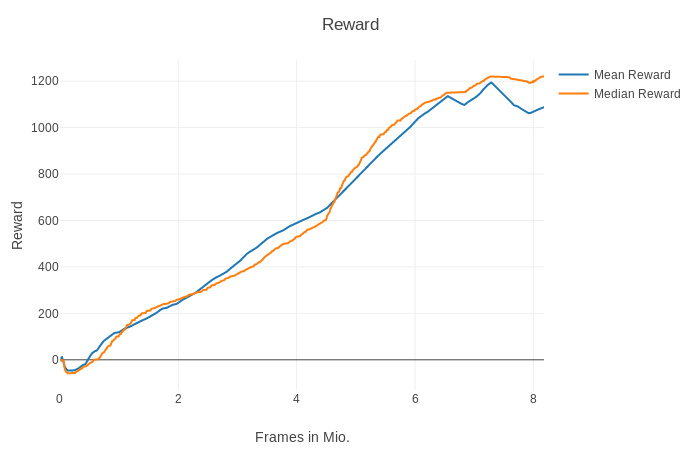
\includegraphics[width=0.9\textwidth]{./latent_i2a_images/MsPacman_dSSM_DET_5rollout.png}
    \end{figure}
\end{frame}


\begin{frame}
	\frametitle{I2A with dSSM-DET environment model MsPacman demo}
\end{frame}


\begin{frame}
	\frametitle{Conclusion}
	\begin{PraesentationAufzaehlung}
		\item Pytorch framework for I2A
		\item Implementation of latent environment model generation
		\item Implementation of I2A using the latent space approach
	\end{PraesentationAufzaehlung}
	
	\bigskip
	Our code will be published on github.\\
	If you are interested send us an email to get the link.
\end{frame}


%Future Work
\begin{frame}
	\frametitle{Potential future work}
	\begin{PraesentationAufzaehlung}
		\item Compact latent representation for both paths
	\item Use GANs for the environment model
	\item Smaller latent space, the latent space in the paper is still pretty large
	
	\item Train environment model together with the policy network.\\
	For complex problems, other state-of-the-art methods may not be good enough to get a representative training set for the environment model training.
	\item Select promising actions to focus rollouts on
	\end{PraesentationAufzaehlung}
\end{frame}


\begin{frame}
	\vspace*{\fill}
	\huge
	\begingroup
	\centering
	Thank you for your attention!
	\endgroup
	\bigskip
	\begingroup
	\centering
	Questions?
	\endgroup
	\normalsize
	\vspace*{\fill}
\end{frame}
